% {{{ Preamble ----------------------------------------------------------------
\documentclass[a4paper,11pt]{article}

% encodings, fonts etc.
\usepackage[utf8]{inputenc}
\usepackage[T1]{fontenc}

% page layout
%\usepackage{a4wide}

% math packages
\usepackage{amsmath, amssymb, amsthm}
\usepackage{mathtools}

% graphics, colors, figures etc.
\usepackage{graphicx}
\usepackage{caption}
\usepackage{subcaption}
\usepackage{float}
\usepackage[export]{adjustbox}
\usepackage{color}



% misc. packages
\usepackage{hyperref}
\usepackage{url}
\usepackage{fancyvrb}

% code etc.
\usepackage{listings}

\usepackage{verbatim}
\usepackage[table,xcdraw]{xcolor}

\definecolor{mygreen}{rgb}{0,0.6,0}
\definecolor{mygray}{rgb}{0.5,0.5,0.5}
\definecolor{mymauve}{rgb}{0.58,0,0.82}

\lstset{%
  backgroundcolor=\color{white},
  basicstyle=\footnotesize\ttfamily,
  breakatwhitespace=true,
  breaklines=true,
  captionpos=t,
  commentstyle=\color{mygreen},
  extendedchars=true,
  keepspaces=true,
  keywordstyle=\color{blue},
  numbers=none,
  numbersep=8pt,
  numberstyle=\tiny\color{mygray},
  rulecolor=\color{black},
  showstringspaces=false,
  showtabs=false,
  stepnumber=1,
  stringstyle=\color{mymauve},
  frame=single,
  frameround=tttt,
  %frame=tb,
  belowskip=-0.2\baselineskip,
}

% mathematics, theorems etc.
\newtheorem*{proposition}{Proposition}
\newtheorem*{lemma}{Lemma}
\newtheorem*{theorem}{Theorem}
\newtheorem{example}{Example}
\theoremstyle{definition}
\newtheorem{definition}{Definition}[section]

% change \qed symbol to black square
\renewcommand\qedsymbol{$\blacksquare$}

% various useful commands
\newcommand{\file}[1]{\texttt{#1}}
\DeclareMathOperator*{\argmin}{arg\,min}
\def\LRA{\hspace{1em}\Leftrightarrow\hspace{1em}}

\newcommand{\type}[1]{\texttt{#1}}
\newcommand{\fun}[1]{\texttt{#1}}

\newcommand{\sfm}{\texttt{scan\_for\_matches}}


% tikz
\usepackage{pgf}
\usepackage{tikz}
\usetikzlibrary{arrows,automata,positioning}

% title page
\title{Kleenex-based approximate pattern matching for DNA analysis}
\author{Anders Kiel Hovgaard \and Daniel Lundberg Pedersen \and Dandan Xue}
\date{January 23, 2017}
% }}} -------------------------------------------------------------------------

\begin{document}

\maketitle

\begin{abstract}
  A master's thesis investigated extending Kleenex with approximate matching by
  rewriting core Kleenex. We design and perform experiments to evaluate the
  performance of this approximate Kleenex implementation as well as three other
  tools for comparison. The experiment results show fairly good runtime
  performance, but they also show that the program is likely impractical at
  this point, because of the problems with long compilation times and the low
  error tolerance that can feasibly be compiled. We present our analysis of
  this problem. We also conduct a survey of approximate matching techniques,
  and at last discuss some possibilities for improving approximate Kleenex.
\end{abstract}
\newpage

\tableofcontents
\newpage

\section{Introduction}

Approximate pattern matching is the problem of finding occurrences of a given
pattern string in a given text string, while allowing some degree of error in
the occurrences. In other words, given some distance metric, the problem is to
find all the occurrences of the pattern in the text including those within a
specified distance of the pattern string. The pattern may denote a single
string, or a set of strings as in the case of a regular expression.

The problem is also known as approximate string matching or searching,
approximate regular string matching, approximate regular substring matching
etc. It is an important problem in many areas, including in bioinformatics
where common tasks involve searching for specific patterns in biological
sequences such as DNA, RNA, and protein, represented as text strings. However
these sequences may contain errors, thus presenting a need for approximate
search techniques.

A number of bachelor theses investigated the use of automata-based techniques
for DNA pattern matching and they compared their implementations to the widely
used domain-specific tool \sfm{}.  This turned out to be just barely
competitive with \sfm{} in some cases. Even more recently, the Kleenex language
and compiler~\cite{grathwohl2016kleenex,soholm2015ordered} was extended to
support approximate matching, and in fact approximate transduction, through
rewriting of core Kleenex programs to express approximate matching as exact
matching~\cite{troelsen2016approximate}. This has indicated even better
performance and even managed to outperform \sfm{} in one case. The evaluation
of this tool with regards to the application of approximate pattern matching in
biological sequences has, however, only been briefly investigated.

This project is about investigating the applicability of Kleenex to the topic
discussed above and comparing it to the NR-grep~\cite{navarro2001nr} program as
well as \sfm{}.

We have found that approximate Kleenex shows a competitive runtime performance
in many case, however often slightly outperformed by NR-grep, and while it is
sometimes outperforming \sfm{}, it does not seem to scale as well with increasing
number of allowed errors $k$. We have also found that the size of the program
generated by approximate Kleenex grows very large as $k$ increases, which is
possibly a major cause of performance degradation.

We also review other existing solutions to the problem of approximate matching
and we discuss potential improvements to the approximate Kleenex program.

%%% Local Variables:
%%% mode: latex
%%% TeX-master: "main"
%%% End:

\section{Background}

This section describes the main background theory of the Kleenex language and
its application to approximate string matching.

\subsection{Transducers}

Kleenex~\cite{grathwohl2016kleenex,soholm2015ordered} is a domain-specific
language for expressing transducers. The concept of a transducer extends that
of a finite automaton to also include output, that is, a finite automaton
either accepts or rejects a string, whereas a transducer produces an output
string in a language over a given output alphabet.

First we define the notion of a finite state transducer, which is essentially
just a nondeterministic finite automaton (NFA) which can also output a symbol
on each transition.

\begin{definition}[FST]
  A \emph{finite state transducer} $\mathcal{T}$ over an input alphabet
  $\Sigma$ and an output alphabet $\Gamma$ is a structure
  $(\Sigma, \Gamma, Q, q^s, q^f, \Delta)$, where
  \begin{itemize}
      \item $Q$ is a finite set of states,
      \item $q^s, q^f \in Q$ are the initial and final states,
        respectively, and
      \item $\Delta \subseteq Q \times \Sigma[\epsilon] \times
        \Gamma[\epsilon] \times Q$ is the transition relation.
  \end{itemize}
\end{definition}

\noindent
Here, $\Sigma[\epsilon]$ denotes the alphabet $\Sigma$ extended with the empty
string $\epsilon$.

Intuitively, there is the following correspondence between the elements of the
transition relation and the transitions in the drawn diagram of the transducer:
\[
  (q, s, t, q') \in \Delta \quad \Leftrightarrow \quad q \xrightarrow{s/t} q'
\]
That is, if $(q, s, t, q') \in \Delta$ then the transducer may transition from
state $q$ to state $q'$ by consuming a symbol $s \in \Sigma[\epsilon]$ and
outputting a symbol $t \in \Gamma[\epsilon]$.

In an NFA, multiple paths may lead to an accepting state for a given input
string, but regardless of which accepting path is chosen, the ouput is the
same. In an FST, on the other hand, the path determines the transduced output,
thus the same input string may produce entirely different outputs depending on
the path chosen.

In order to disambiguate between different transductions of the same input
string, we introduce the notion of a normalized
FST~\cite{grathwohl2016kleenex}. To facilitate this, we also introduce two new
symbols $\epsilon_0$ and $\epsilon_1$. Both denote the empty string, but they
serve to distinguish between nondeterministic $\epsilon$-transitions.

\begin{definition}[NFST]
  A \emph{normalized finite state transducer} is a deterministic FST,
  $\mathcal{T} = (\Sigma[\epsilon_0,\epsilon_1], \Gamma, q^s, q^f, \Delta)$,
  with the constraint that for any state $q$ in $Q$, $q$ is either a choice
  state, a skip state, a symbol state, or the final state.
\end{definition}

The notions of choice, skip, or symbol states are perhaps best conveyed by
illustration, as shown in Figure~\ref{fig:nfst-states}.

\begin{figure}[!ht]
  \centering
  \begin{subfigure}[b]{0.3\textwidth}
    \centering
    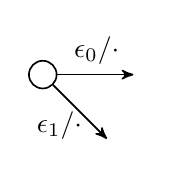
\begin{tikzpicture}[->,>=stealth',shorten >=1pt,auto,node distance=1.0cm,
      semithick, main/.style={circle,draw,minimum width=10pt}]
        \node[main] (q0) {$ $};
        \node       (q1) [right = of q0] {};
        \node       (q2) [below right = of q0] {};
        \path (q0) edge node {$\epsilon_0/\cdot$} (q1)
              (q0) edge node [below left = -2mm, swap]
                   {$\epsilon_1/\cdot$} (q2);
    \end{tikzpicture}
    \caption{A choice state.}
  \end{subfigure}
  ~
  \begin{subfigure}[b]{0.3\textwidth}
    \centering
    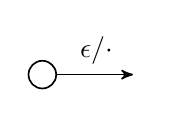
\begin{tikzpicture}[->,>=stealth',shorten >=1pt,auto,node distance=1.0cm,
        semithick, main/.style={circle,draw,minimum width=10pt}]
        \node[main] (q0) {$ $};
        \node       (q1) [right = of q0] {};
        \path (q0) edge node        {$\epsilon/\cdot$} (q1);
    \end{tikzpicture}
    \caption{A skip state.}
  \end{subfigure}
  ~
  \begin{subfigure}[b]{0.3\textwidth}
    \centering
    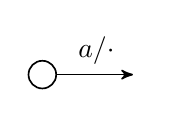
\begin{tikzpicture}[->,>=stealth',shorten >=1pt,auto,node distance=1.0cm,
      semithick, main/.style={circle,draw,minimum width=10pt}]
        \node[main] (q0) {$ $};
        \node       (q1) [right = of q0] {};
        \path (q0) edge node {$a/\cdot$} (q1);
    \end{tikzpicture}
    \caption{A symbol state.}
  \end{subfigure}
  \caption{Illustration of choice states, skip states, and symbol states.}
  \label{fig:nfst-states}
\end{figure}

Thus, the set of symbols that any state has transitions on, i.e. the support of
the state, is either just $\epsilon$ (for skip states), exactly
$\{\epsilon_0, \epsilon_1\}$ (for choice states), exactly one $a \in \Sigma$
(for symbol states), or $\emptyset$ in the case of the final state. The idea is
that $\epsilon_0$ and $\epsilon_1$ imposes an ordering on the nondeterministic
transitions of the choice states, with $\epsilon_0$ being preferred over
$\epsilon_1$. In order to define this more precisely, we need a few more
definitions.

A \emph{path} in a transducer is a sequence of consecutive
transitions
\[
  q_0 \xrightarrow{x_1/y_1} q_1 \xrightarrow{x_2/y_2} \dots
  \xrightarrow{x_n/y_n} q_n
\]
which can be written more compactly as
\[
  q_0 \xrightarrow{x/y} q_n
\]
where $x = x_1x_2 \dots x_n$ is the input string and $y = y_1y_2 \dots y_n$ is
the output string of the path.

Define a mapping from $\Sigma[\epsilon, \epsilon_0, \epsilon_1]$ to
$\mathbf{2}[\epsilon]$, i.e. the binary alphabet with $\epsilon$, mapping
$\epsilon_0$ to $0$, $\epsilon_1$ to $1$, and any other symbol to
$\epsilon$. This naturally extends to a mapping from strings over the extended
input alphabet to strings of bits. The \emph{greedy disambiguation strategy} of
an NFST is the strategy that chooses the path with the lexicographically least
input bit string, as given by this mapping.

% TODO: consider including example
% TODO: consider talking about oracle and action automata


\subsection{Kleenex}

As mentioned previously, Kleenex is a domain-specific programming language for
specifying finite transducers, and specifically the core language directly
encodes NFSTs.

\subsubsection{Core Kleenex}

\begin{definition}[Core Kleenex~\cite{grathwohl2016kleenex}]
  A core Kleenex program is a list of definitions of the form $N := t$, where
  $t$ is generated by the grammar
  \[
    t ::= \epsilon \;|\; N \ |\ \mathtt{a}\; N' \;|\; \mathtt{"b"} N' \;|\;
    N_0|N_1
  \]
  and $a \in \Sigma, b \in \Gamma$, for some given input alphabet $\Sigma$ and
  output alphabet $\Gamma$.
\end{definition}

A core Kleenex program is transformed to an NFST in a direct and
straightforward way: Each nonterminal $N, N', \dots$ maps to a state in the
transducer, the set of states is extended with a final state $q^f$, and each
core Kleenex definition maps to one or two transitions in the transducer as
follows:

\begin{center}
  \begin{tabular}{|l|l|}
    \hline
    $N := \epsilon$       & $N \xrightarrow{\epsilon/\epsilon} q^f$   \\
    \hline
    $N := N'$             & $N \xrightarrow{\epsilon/\epsilon} N'$    \\
    \hline
    $N := \mathtt{a}N'$   & $N \xrightarrow{a/\epsilon} N'$           \\
    \hline
    $N := \mathtt{"b"}N'$ & $N \xrightarrow{\epsilon/b} N'$           \\
    \hline
    $N := N_0 \;|\; N_1$  & $N \xrightarrow{\epsilon_0/\epsilon} N_0$ \\
                          & $N \xrightarrow{\epsilon_1/\epsilon} N_1$ \\
    \hline
  \end{tabular}
\end{center}

\subsubsection{Streaming simulation and determinization}

Grathwohl et al.~\cite{grathwohl2016kleenex}, as well as Søholm and
Tørholm~\cite{soholm2015ordered}, describe how a normalized FST, respectively
an ordered finite transducer (an alternative model), can be simulated in a
streaming fashion using \emph{path-tree simulation}. This algorithm maintains a
structure called a \emph{path tree}, a binary tree which plays a similar role
to the set of active states in NFA simulation, but it also maintains the paths
from the initial state to all the states reachable on the current prefix of the
input. The output produced in the stem of the path tree, that is, the path from
the root to the first branching node, may be output immediately, thus enabling
streaming transduction.

A path tree may be \emph{reduced} by pruning duplicate leafs with
lexicographically larger bit strings, since they will not be preferred by the
greedy disambiguation strategy, and by merging non-branching nodes and
concatenating their outputs.

Since the number of reduced path trees is finite~\cite{soholm2015ordered}
(ignoring output), these may be precomputed to determinize the NFST. A
\emph{streaming string transducer} (SST) is a deterministic automaton with
abstract states corresponding to the reduced path trees, transitions
representing how the reduced path trees transform on given input, and registers
which store the outputs associated with each node in the path tree.


\subsection{Approximate matching and transduction in Kleenex}
\subsubsection{Approximate pattern matching}
Approximate pattern matching is the pattern matching problem that allows errors. The error metrics or the distance between strings can affect the result of approximate matching a lot. The most common three of error metrics are Hamming distance, Longest common subsequence distance(LCS) and Levenshtein distance. The errors types are usually these three: replacement (or substitution), insertion and deletion.

% TODO: consider some formal definition of approximate matching 

\subsubsection{Aprroximate Kleenex} \label{sec:approx-kleenex}
Peter Troelsen describes, in his master's
thesis~\cite{troelsen2016approximate}, an approach to approximate transduction
using Kleenex, by rewriting of core Kleenex programs. This is done by
expressing approximate matching as exact matching through program
transformation. A core Kleenex term that accepts strings of some language $L$
is transformed to another term which accepts strings from $L$ as well as any
string with a distance of at most $k$ to some string in $L$, given some
distance metric.

Troelsen's approach is purely a transformation of the core language, so the
rest of the compilation process and optimizations of the Kleenex compiler
remains unchanged. This means that the transformed transducer will also be
compiled to a streaming string transducer, thus harnessing the high performance
at runtime, but also suffering the potentially high increase in automata size
with the determinization of the transducer. For this reason, one can speculate
that an implementation which works at a deeper level of the compilation process
may be able to optimize things and reduce the number of generated states and
transitions.

% for instance by counting the errors instead of encoding the number of allowed
% errors directly in the program grammar

As an example of the core Kleenex rewriting and its influence on the
transducer, consider rewriting the following program to accept up to two
mismatches (i.e. a Hamming distance of $k=2$):
\begin{align*}
  N   &:= N' | N''      \\
  N'  &:= \mathtt{a} N  \\
  N'' &:= \epsilon
\end{align*}
In its current form, this program accepts strings denoted by the regular
expression $\mathtt{a^*}$, and we intent to extend it to allow at most 2
symbols which are not $\mathtt{a}$. Using Troelsen's $k$-fold rewrite for
Hamming distance, we obtain the following program:
\begin{align*}
  N_0   &:= N'_0 \;|\; N''_0  &  N_1   &:= N'_1 \;|\; N''_1           & N_2   &:= N'_2 \;|\; N''_2           \\
  N'_0  &:= \mathtt{a} N_0    &  N'_1  &:= \mathtt{a} N_1 \;|\; . N_0 & N'_2  &:= \mathtt{a} N_2 \;|\; . N_1 \\
  N''_0 &:= \epsilon          &  N''_1 &:= \epsilon                   & N''_2 &:= \epsilon
\end{align*}

The nonterminal $N_2$ now accepts 2 mismatches. Actually, $N'_1$ and $N'_2$
would need to be converted into alternations between two new nonterminals for
this to be a core Kleenex program, but this only adds a constant number of new
definitions. There also needs to be added a new start symbol with nested
alternations indicating a preference for which $N_i$ to start with.

The transducers for the original program and the rewritten approximate program
have been visualized using the built-in functionality of the Kleenex compiler
and are attached in Appendix~\ref{app:approx-kleenex-example}.

This rewritten program only allows up to $k$ mismatches. The program would be
larger if it also needed to support insertions and deletions, albeit only by a
constant factor~\cite{troelsen2016approximate}. The program grows rather large
as $k$ increases. This issue will be further discussed later on in this report.

%%% Local Variables:
%%% mode: latex
%%% TeX-master: "main"
%%% End:

\section{Experiments}

\subsection{Introduction to the tools}
\subsubsection{Python (\texttt{regex})}
The \texttt{regex}\footnote{\url{https://pypi.python.org/pypi/regex}} Python
module is intended to replace the current \texttt{re} module at some point. It
is a fairly fully fledged regular expression module, that also supports
approximate matching. Because of this and the ease of creating the necessary
scripts we chose to include it in the benchmarks. Unfortunately, there is
little information, other that the source code, about the theoretical
background or the inner workings of this implementation.

\subsubsection{Approximate Kleenex}
Approximate matching was introduced to Kleenex by P. Troelsen in his master's
thesis~\cite{troelsen2016approximate}. As discussed previously, this is
accomplished by rewriting the core program terms to allow for a given number of
errors in the match, that is, to express the approximate matching as exact
matching.

\subsubsection{Scan For Matches}
Scan For Matches\footnote{\url{http://blog.theseed.org/servers/2010/07/scan-for-matches.html}}
(SFM)~\cite{dsouza1997searching} is an approximate pattern matching tool
specifically designed for matching biological sequences such as DNA, RNA, and
protein. It is written in C and has a bunch of nucleotide and protein specific
niceties that the other tools do not, such as using FASTA files directly, and
support for matching reverse complements (matching the DNA complement of a
previously occurred subpattern in reverse, e.g. corresponding to an RNA hairpin
loop).

\subsubsection{NR-grep}
NR-grep~\cite{navarro2001nr} is a fast pattern matching tool, similar to
\texttt{grep}, that is made to be effecient for complex pattern, and it also
supports approximate matching.


\subsection{Experiment setup and benchmark description}
The experiments where run on the \texttt{gpu02} machine.
\begin{description}
    \item[CPU] Intel Xeon E5-2650 v2 (2.60 GHz).
    \item[RAM] 128 GB.
    \item[Disk] KU network share.
\end{description}

The data set used for the benchmark is from
\url{ftp://ftp-trace.ncbi.nih.gov/1000genomes/ftp/technical/reference/human_g1k_v37.fasta.gz}
and is 2.9 GBs uncompressed, for most of the benchmarks we used a file where we
stripped the newlines, so they would not count as an error, except for the
NR-grep trails since it was not too happy about lines longer than $2^{16}$.

\subsubsection{Patterns used}
We have made a number of patterns to benchmark the different tools, they are
represented here in the Kleenex syntax, with $k$ being the allowed number of
substitutions going from 0 up to 5 (if possible). They are not all possible in
all of the tools, only Kleenex has support for all the patterns. Also we search
for the pattern, not just plain string matching, so in Kleenex we had to add an
alternation and a star, to discard any input that did not match the pattern.

\texttt{/TGCAAGCGTTAAT/<$k$>} - Short - A simple fairly short pattern with
nothing but a character string.

\texttt{/GCCCAGAGAACTTTCAGGATGACACCAGCAAGG/<$k$>} - Long - A longer simple
pattern it is only 33 characters long because it was the longest we could
compile a Kleenex program for with $k \leq 2$

\texttt{(/GCCCAGAGA/|/ACTTTCAGGA/)<$k$>} - Alternation - An alternation with a
simple fairly short pattern on each side of the alternation.

\texttt{(/[ACGT]/\{5,15\} /TGCAAGCGTTAAT/)<k>} - Ranges - A small pattern with
a ranges of repetitions, followed by another fairly short pattern.

\subsection{Results}
In Figure \ref{fig:short}, we have the runtimes for the \textit{Short} pattern
with the different tools. What we see is that \texttt{regex} seems to be quite
far outmatched by all the other tools, which seems to by a general thing, the
cause for being so far behind, can probably partly be blamed on the Python
scripts read the entire file in to memory before beginning to search for the
pattern. But overall \texttt{regex} does not seem to have too bad a complexity
with respect to $k$. For the rest of the tools they are fairly close in
performance with SFM being the worst in low $k$ but having a seemingly near
constant complexity with respect to $k$ and performing better for larger $k$.
NR-grep while having the advantage of not having a single line file, gives the
best results here for smaller $k$, but does have some wiered behaviour with it
being better for $k=5$ and for $k=4$. Finally Kleenex performes quite well
beating out SFM but not NR-grep, to begin with, but does really bad once we hit
$k=3$, the reason for this sudden performance hit is likely due to caching
issues, that are grounded in the executable size being 11MB.

Figures \ref{fig:long} and \ref{fig:alternation} show fairly similar results to
to that of Figure \ref{fig:short}, which suggest that none of the tools do
anything special that would change their relative performace.

Finally Figure \ref{fig:ranges} show Kleenex performing quite bad when having a
range to match, especially when the large executable size for $k=1$ kicks in.
Whereas \texttt{regex} has a similar performance to the other benchmarks.

\begin{figure}[!ht]
  \centering
  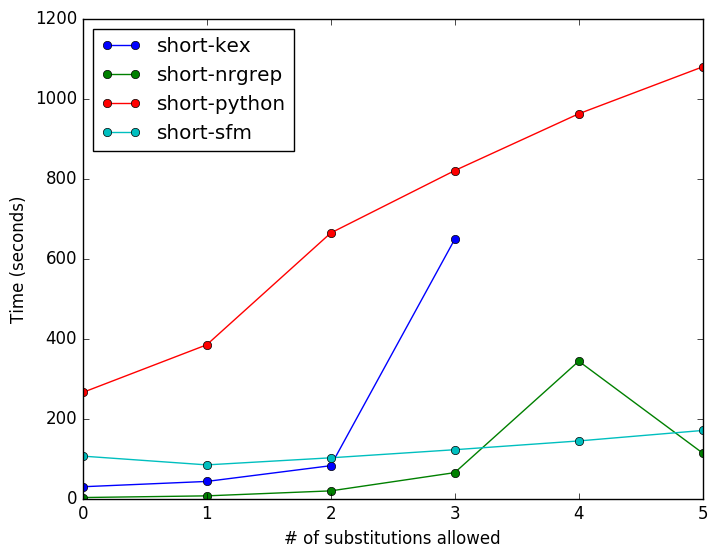
\includegraphics[width=0.9\textwidth]{images/short.png}
  \caption{Execution times for approximate Kleenex, NR-grep, Python's
    \texttt{regex} module, and \texttt{scan\_for\_matches}, when searching for
    the pattern \texttt{/TGCAAGCGTTAAT/<$k$>} for $k=0..5$.}
  \label{fig:short}
\end{figure}

\begin{figure}[!ht]
  \centering
  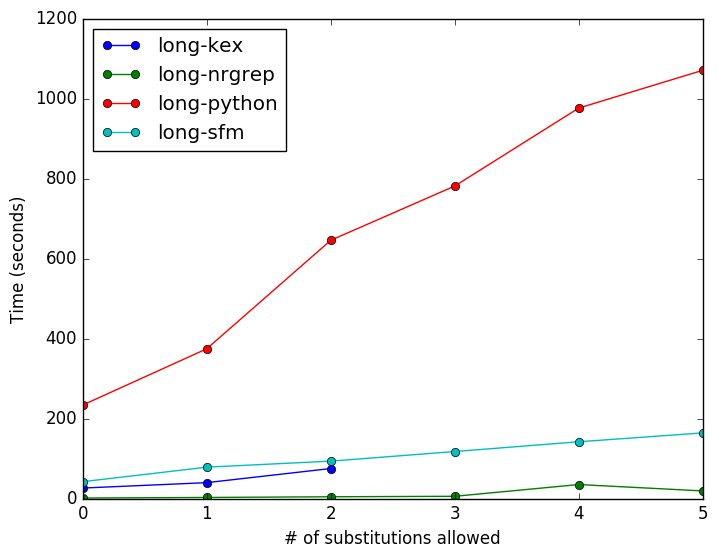
\includegraphics[width=0.9\textwidth]{images/long.png}
  \caption{Execution times for the evaluated tools when searching for the
    pattern \texttt{/GCCCAGAGAACTTTCAGGATGACACCAGCAAGG/<$k$>} for $k=0..5$.}
  \label{fig:long}
\end{figure}

\begin{figure}[!ht]
  \centering
  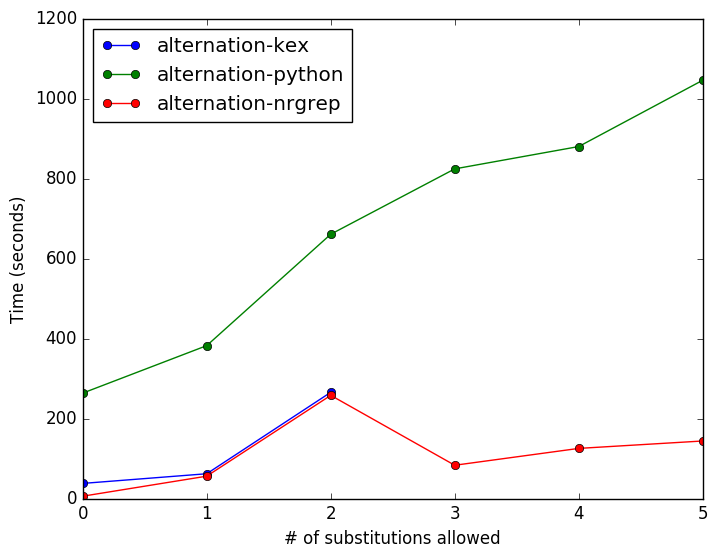
\includegraphics[width=0.9\textwidth]{images/alternation.png}
  \caption{Execution times for the evaluated tools when searching for the
    pattern \texttt{(/GCCCAGAGA/|/ACTTTCAGGA/)<$k$>} for $k=0..5$.}
  \label{fig:alternation}
\end{figure}

\begin{figure}[!ht]
  \centering
  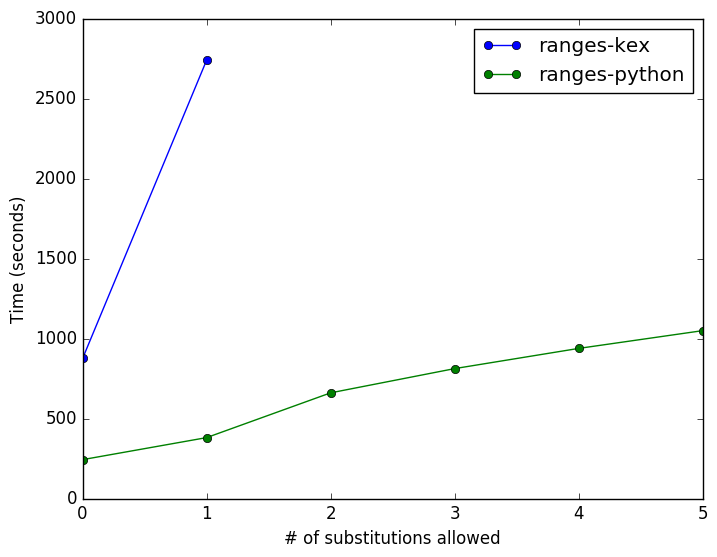
\includegraphics[width=0.9\textwidth]{images/ranges.png}
  \caption{Execution times for the evaluated tools when searching for the
    pattern \texttt{(/[ACGT]/\{5,15\} /TGCAAGCGTTAAT/)<$k$>} for $k=0..5$.}
  \label{fig:ranges}
\end{figure}

\begin{figure}[!ht]
    \centering
    \begin{tabular}{l|rrrrr}
                    & 0     & 1     & 2     & 3\\\hline
        Short       & 23    & 89    & 716   & 11,000\\
        Long        & 23    & 192   & 1,700 & N/A\\
        Alternation & 32    & 234   & 2,800 & N/A\\
        Ranges      & 92    & 21,000& N/A   & N/A\\
    \end{tabular}
    \caption{Size(KB) of the executables generated by Kleenex for the patterns
    and different $k$.}
    \label{fig:exec}
\end{figure}

\subsubsection{Remarks}
NR-grep is capable of searching in lines that are longer than $2^{16}$ but it
outputs a bunch of warnings cluttering output, and also has some wierd runtimes
as seen in Figure \ref{fig:nr-longline}, and this is without having checked if
it finds the correct number of matches.

Also SFM does not seem to support approximate matching for alternations, as we
could not get the pattern to compile with the error values added.

\begin{figure}[!ht]
    \centering
    \begin{tabular}{l|rrrrr}
        $k$ & Time (s)\\\hline
        0   & 4.59\\
        1   & 43.32\\
        2   & 1185.80\\
        3   & 1323.27\\
        4   & 906.27\\
        5   & 30.04\\
    \end{tabular}
    \caption{Run time for NR-grep with a single long line.}
    \label{fig:nr-longline}
\end{figure}


%%% Local Variables:
%%% mode: latex
%%% TeX-master: "main"
%%% End:

\section{Survey of approximate matching techniques}
The approximate matching problem is in general more complicated than the exact matching problem. We can consider exact matching problems as a subset of approximate matching problems with an error of 0. We should note that the problem set will also change a lot if we use a different error metric(such as Levenshtein distance or Hamming distance) or a different model of errors (such as insertation, deletion or transition). The time complexity of many efficient exact matching algorithms that work as simulating DFAs, such as the Knuth--–Morris--–Pratt algorithm, will become exponential as the number of errors grows if we just convert the NFAs that accepts the pattern with errors into DFAs to be applied in these algorithms. 

From now on we denote the pattern string with $pat$ and the text string with $txt$ and  the lengths of them are $m$ and $n$ respectively.

\subsection{Dynamic programming}

One of the classical solutions to approximate matching is to use dynamic programming. This method is simple and easy to be implemented by programming. It has been proved that if the alphabet is of a constant size, approximate string matching with $k$ errors can be solved in $O(kn)$ time\cite{crochemore-jewels}. The investigation of the theory background is heavy and can be left as future work.

Here we present an idea of how to match a pattern with the Levenshtein distance by dynamic programming. Informally, the Levenshtein distance between two strings is the minimum number of edits(including replacement, insertion and deletion) that requires to change one string into the other. The problem above can be considered as filling in a matrix of size $m\times n$. In such a matrix, an element [$i$+1,$j$+1] ($i$ and $j$ denote the number of row and column respectively in the matrix) is filled with the value [$i$,$j$] if $pat$[$i$+1] is the same with $txt$[$j$+1]; otherwise the sum of 1 and the minimum of [$i$,$j$],[$i$,$j$+1] and [$i$+1,$j$], which indicates a replacement, a deletion and an inseration respectively. We show an example of such a problem.

\begin{example} \emph{Dynamic programming solving approximate matching with the Levishtein distance of 1 for pattern "abc" and text "abaab".}

\begin{table}[H]
	\centering
\begin{tabular}{|c|c|c|c|c|c|}
	\hline
	\multicolumn{1}{|l|}{}            & \multicolumn{1}{l|}{}    & \multicolumn{1}{l|}{\textbf{a}}   & \multicolumn{1}{l|}{\textbf{b}}   & \multicolumn{1}{l|}{\textbf{a}} & \multicolumn{1}{l|}{\textbf{a}} \\ \hline
	& \textbf{0}               & 1                                 & 2                                 & 3                               & 4                               \\ \hline
	\textbf{a}                        & 1                        & {\color[HTML]{000000} \textbf{0}} & 1                                 & {\color[HTML]{333333} 2}        & {\color[HTML]{333333} 3}        \\ \hline
	\textbf{b}                        & 2                        & 1                                 & \textbf{0}                        & {\color[HTML]{333333} 1}        & {\color[HTML]{333333} 2}        \\ \hline
	{\color[HTML]{333333} \textbf{c}} & {\color[HTML]{333333} 3} & {\color[HTML]{333333} 2}          & {\color[HTML]{32CB00} \textbf{1}} & {\color[HTML]{000000} 1}        & {\color[HTML]{333333} 2}        \\ \hline
\end{tabular}
\end{table}
	\label{fig:dynap}
 \end{example}
 
If we look at the last row of this matrix, the filled values from left to right show us how the Levinshtein distance changes between the pattern and the text we have read. When we read in the second character of the text, i.e. $b$, a match is found, that is $ab$ matches $abc$ with one error. The numbers in bold show us the path of this match: two diagnoal steps with no increase on the value mean two exact matchs of single character (i.e., matches of $a$ and $b$) and one vertical step means an insertation (i.e., insertion of $c$). 

Dynamic programming is simple, practical and easy to be extended to support more functionalities such as specifying the number of each type of errors, which can be implemented by finding a particular path in the matrix as we have shown above. It is likely that our experiment tools such as Python {\tt regex} and Scan\_for\_matches are based on this method as the time complexity appears close to linear. As there is no documentation or describution of what the approximate matching algorithms are used in these tools, this can be left as future work for further investegation.

\subsection{Automaton simulation}
Another classical approach is to use automaton simulation. The algortihm BNDM  (we will explain later) over which NR-grep is built is basically a simulation of an NFA. 

From the experiment results shown in the previous section, we find NR-grep has the best performance in average in our various test cases. This is not surprising because NR-grep implemented different efficient algorithms for various pattern matching problems as well as a good software design. We present some important techniques of approximate matching as well as efficient matching algorithms that used in NR-grep.

\subsubsection{Bit-parallelism}

From NR-grep's perspective, the patterns are classified into three levels: simple patterns, extended patterns and regular experssions. Different patterns are applied  different algorithms to make sure that the problem can be solved in the most efficient way. The name of this tool comes from "nondeterministic reverse $grep$", which indicates this tool can simulate NFAs instead of converting them to DFAs. The algorithm of  simulating NFAs used in NR-grep is called $\operatorname{Shift-Or}$. This algorithm is based on an approach called $\operatorname{bit-parallelism}$, which takes advantage of the parallelism of bit operations inside a computer word. A variant of Shift-Or that is easier to explain is $\operatorname{Shift-And}$ algorithm. We first show how this algorithm works. 

Given both the pattern and the text in the alphabet $\Sigma$ with a size $|\Sigma|$, first we build a table $B$ in which for each character in $\Sigma$ stores a bit mask $b_m...b_1$. For a character $char$ in $pat$ with an index $i$ (1-indexed), set the $\operatorname{(m-i-1)}$ bit of the mask in B[$char$]. The following example shows a bit mask table for the pattern "abc".


\begin{example}\emph{The bit mask table for pattern "abc", assuming $\Sigma$ = \{a,b,c,d\}.}

\begin{table}[H]
	\centering
	\begin{tabular}{|c|c|c|c|}
		\hline
		index      & 1                        & 2                        & 3                        \\ \hline
		\textbf{a} & 0                        & 0                        & {\color[HTML]{3531FF} 1} \\ \hline
		\textbf{b} & 0                        & {\color[HTML]{3531FF} 1} & 0                        \\ \hline
		\textbf{c} & {\color[HTML]{3531FF} 1} & 0                        & 0                        \\ \hline
		\textbf{d} & 0                        & 0                        & 0                        \\ \hline
	\end{tabular}
	\label{table-bitmask}
\end{table}
\end{example}

We use a computer word $D = d_m...d_1$ to store the current active state (or the current matching position in the pattern) with an initial value of all bits 0. During the searching process, $D$ is updated with the following formula: 
$$D' \leftarrow ((D << 1) \ | \ 0^{m-1}1) \ \& \ B[t_j]$$
where $t_j$ is the next text character.  When the $d_m$ bit in $D$ is set, we report a match. 

One of the advantages of the $\operatorname{Shift-And}$ algorithm is that it is easy to be extended to handle classes of characters, which is helpful for approximate matching. 
For example, we can now search for the pattern "ab."\footnote{ We use symbol '.' in this report to stand for a wildcard.}, which can be considered as the pattern "abc" allowing at most one replacement error at the third character by just setting the $\operatorname{(m-3+1)}$ bit of all the characters in the bit mask table, as the following example shows. 

\begin{example}\emph{The bit mask table for pattern "ab."}.
	\begin{table}[H]
		\centering
		\begin{tabular}{|c|c|c|c|}
			\hline
			index      & 1                        & 2                        & 3                        \\ \hline
			\textbf{a} & {\color{red} 1}                   & 0                        & {\color[HTML]{3531FF} 1} \\ \hline
			\textbf{b} &  {\color{red} 1}                    & {\color[HTML]{3531FF} 1} & 0                        \\ \hline
			\textbf{c} & {\color[HTML]{3531FF} 1} & 0                        & 0                        \\ \hline
			\textbf{d} &{\color{red} 1}                    & 0                        & 0                        \\ \hline
		\end{tabular}
		\label{table-bitmask2}
	\end{table}
\end{example}

With this new bit mask table, searching for the pattern "ab.", or more generally a pattern that contains wildcards, will be just the same time complexity as search for "abc". 
%We can also find that an error of insertion can be dealt with by adding a new row of all 1s in the bit mask table and a deletion is just removing one row. 
 
\subsubsection{BNDM algorithm}
As we know, many efficient exact pattern matching algorithms, such as the Knuth--–Morris--–Pratt and the Boyer-Moore algorithm, utilize a trick of skipping characters. It is aslo possible to combine the $\operatorname{bit-parallelism}$ approach with the ability of skipping characters to achieve an even more efficient algorithm. This idea is implemented in the $BNDM$ algorithm as we have introduced before. BNDM uses $\operatorname{Shift-Or}$ instead of $\operatorname{Shift-And}$, a variant of $\operatorname{Shift-And}$ that uses the following state updating formula:  
$$ D' \leftarrow  (D \ \& \ B[t_j]) << 1 .$$ The algorithm that is adapted in BNDM for skipping charaters is from the Boyer-Moore or the BDM families\cite{crochemore1994text}.


\subsubsection{NFA simulation}
As we have shown above, bit-parallelism can deal with single error efficiently.
Now we present how bit-parallelism can be used to simulate NFAs for approximate matching. 

Consider the pattern "ab" allowing one error, we can build an NFA to simulate it as the follow figure shows.

\begin{figure} [H]
\begin{center}
	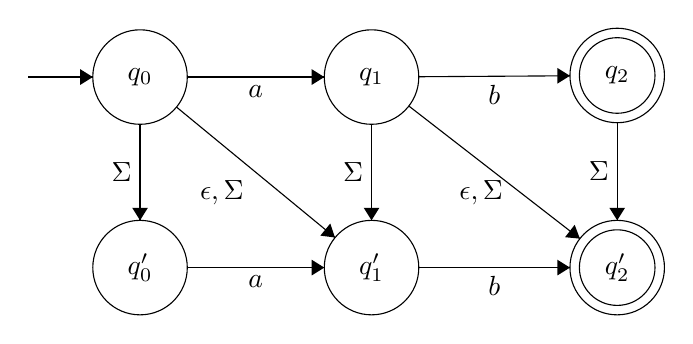
\begin{tikzpicture}[scale=0.2]
	\tikzstyle{every node}+=[inner sep=0pt]
	\draw [black] (18.3,-25.8) circle (3);
	\draw (18.3,-25.8) node {$q_0$};
	\draw [black] (33,-25.8) circle (3);
	\draw (33,-25.8) node {$q_1$};
	\draw [black] (18.3,-37.9) circle (3);
	\draw (18.3,-37.9) node {$q_0'$};
	\draw [black] (33,-37.9) circle (3);
	\draw (33,-37.9) node {$q_1'$};
	\draw [black] (48.6,-25.7) circle (3);
	\draw (48.6,-25.7) node {$q_2$};
	\draw [black] (48.6,-25.7) circle (2.4);
	\draw [black] (48.6,-37.9) circle (3);
	\draw (48.6,-37.9) node {$q_2'$};
	\draw [black] (48.6,-37.9) circle (2.4);
	\draw [black] (11.2,-25.8) -- (15.3,-25.8);
	\fill [black] (15.3,-25.8) -- (14.5,-25.3) -- (14.5,-26.3);
	\draw [black] (21.3,-25.8) -- (30,-25.8);
	\fill [black] (30,-25.8) -- (29.2,-25.3) -- (29.2,-26.3);
	\draw (25.65,-26.3) node [below] {$a$};
	\draw [black] (21.3,-37.9) -- (30,-37.9);
	\fill [black] (30,-37.9) -- (29.2,-37.4) -- (29.2,-38.4);
	\draw (25.65,-38.4) node [below] {$a$};
	\draw [black] (18.3,-28.8) -- (18.3,-34.9);
	\fill [black] (18.3,-34.9) -- (18.8,-34.1) -- (17.8,-34.1);
	\draw (17.8,-31.85) node [left] {$\Sigma$};
	\draw [black] (33,-28.8) -- (33,-34.9);
	\fill [black] (33,-34.9) -- (33.5,-34.1) -- (32.5,-34.1);
	\draw (32.5,-31.85) node [left] {$\Sigma$};
	\draw [black] (36,-25.78) -- (45.6,-25.72);
	\fill [black] (45.6,-25.72) -- (44.8,-25.22) -- (44.8,-26.22);
	\draw (40.8,-26.26) node [below] {$b$};
	\draw [black] (36,-37.9) -- (45.6,-37.9);
	\fill [black] (45.6,-37.9) -- (44.8,-37.4) -- (44.8,-38.4);
	\draw (40.8,-38.4) node [below] {$b$};
	\draw [black] (20.62,-27.71) -- (30.68,-35.99);
	\fill [black] (30.68,-35.99) -- (30.38,-35.1) -- (29.75,-35.87);
	\draw (23.49,-32.34) node [below] {$\epsilon, \Sigma$};
	\draw [black] (48.6,-28.7) -- (48.6,-34.9);
	\fill [black] (48.6,-34.9) -- (49.1,-34.1) -- (48.1,-34.1);
	\draw (48.1,-31.8) node [left] {$\Sigma$};
	\draw [black] (35.37,-27.64) -- (46.23,-36.06);
	\fill [black] (46.23,-36.06) -- (45.9,-35.18) -- (45.29,-35.97);
	\draw (39.96,-32.35) node [below] {$ \epsilon,\Sigma$};
	\end{tikzpicture}
\end{center}
\caption{An NFA accepting the pattern "ab" with at most one error. The label $\epsilon,\Sigma$ on the diagnoal arrows means both $\epsilon$ and $\Sigma$ can be accepted.}
\label{fig:nfa"ab"}
\end{figure}
 
In Figure \ref{fig:nfa"ab"}, the last state of each row stands for a state that accepts $r$ errors where $r$ is the index of the row (0-indexed). That is, in our example, the state $q_2$ accepts "ab" with no errors and $q_2'$  with exact one error. The vertical arrows represent insertion, and the diagonal arrows with the label $\epsilon$ and $\Sigma$ stand for deletion and replacement respectively. For any other pattern with $k$ errors, we could also build an NFA to accept it in such a way by iteration. It is worth noting that the number of states in the NAF built in this way increases linearly with the number of errors.

The technique stores each row in a machine word, say $R_i$ for row $i$, just as the $D$ we have seen in $\operatorname{Shift-And}$.
The formulars for updating these words are listed below:

\begin{align*}
&R_0' \leftarrow  ((R_0 << 1) \ |\ 0^{m-1}) \ \& \ B[t_j] \\
&for \ i \in 1...k \ do:  \\
&\ \ \ \ R_i' \leftarrow ((R_i << 1) \ \& \ B[t_j] ) \ |\ R_{i-1} \ | \ (R_{i-1} << 1 ) \ |\ (R_{i-1}' << 1)
\end{align*}

These formulars show us one case of how bit-parallelism simulate an NFA. $R_0$ is updated just as we have done with $D$ in $\operatorname{Shift-And}$. In the formular for updating $R_i$, the first element (i.e., $((R_i << 1) \ \& \ B[t_j] ) $ ) is similar to the one for updating $R_0$  but without the $OR$ operation with $0^{m-1}$ because $R_i$ can not be an initial state that has a self-loop. The second is the old value of its upper row, which corresponds to a vertial arrow in the NFA. Similarly, the third stands for a replacement and the fourth a deletion. When we detect that $R_k \& 10^{m-1}$ is not zero, a match is reported.  

As we can see from the above updating formulas, each updating is just bitwise operation hence constant time. So this simulation should be only linear time complexity increased, i.e, $O(k)$, compared with the simulation of exact matching of the same pattern.
 

\subsubsection{Splitting technique}
An important property of $k$ errors approximate matching has been found that if we split the pattern into $k+1$ pieces then there must be at least one piece that has no errors\cite{wu1992}. Note that this property only works for an error model of insertion, replacement and deletion. With this property, the approximate matching problem can be reduced to the multi-pattern matching problem with an extra verification, which is to check if the surrounding text of these pieces can be a match of the whole pattern that allows $k$ errors. This technique is also employed in NR-grep. 

\section{Problem analysis}

\subsection{Analysis of automata generated by approximate Kleenex}
To try to get an idea of what problems approximate Kleenex has, we tried to do
some visualization of the following simple program, and also
trying to manually generate the transducer to see if there was something it did
wrong.
\begin{center}
    \texttt{main := (/AT/<1> | ~/./)*}
\end{center}

Which translates to the following core Kleenex program,
\begin{align*}
    N0      &:= N1\ |\ N7\\
    N1      &:= N2-1\ |\ N6\\
    N2_0    &:= \texttt{A}\ N3_0\\
    N3_0    &:= \texttt{"A"}\ N4_0\\
    N4_0    &:= \texttt{T}\ N5_0\\
    N5_0    &:= \texttt{"T"}\ N0\\
    N2_1    &:= \texttt{A}\ N3_1\ |\ \texttt{.}\ N3_0\\
    N3_1    &:= \texttt{"A"}\ N4_1\\
    N4_1    &:= \texttt{T}\ N5_1\ |\ \texttt{.}\ N5_0\\
    N5_1    &:= \texttt{"T"}\ N0\\
    N6      &:= \texttt{.}\ N0\\
    N7      &:= \epsilon\\
\end{align*}
Figure \ref{fig:oft} and Figure \ref{fig:sst} repectively show the OFT and SST
of the program. So far we could see those two correspond correctly to the
program. Though it is possibly to improve the OFT by hand, as seen in Figure
\ref{fig:opt}, how this translates to the SST is a bit harder to see, as the
SST already only has 5 states, but the transition relation is quite complex,
and there are some transitions that could be merged. If these optimizations
could be generalized, they could probably help immensely on some of the program
sizes and performance, since from a random state out of $2556$ in our Ranges
pattern with $k = 1$ we see a single transition executing 82 lines of C code to
make the transition, and the state overall being 650 lines long.

\begin{figure}[!hb]
  \centering
  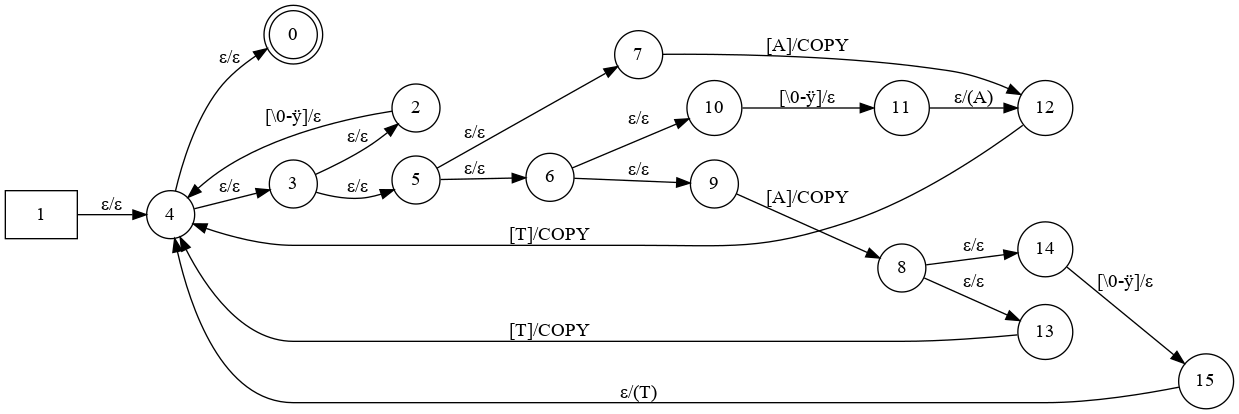
\includegraphics[width=0.9\textwidth]{images/oft.png}
  \caption{OFT of the simple approximate Kleenex program}
  \label{fig:oft}
\end{figure}
\begin{figure}[!hb]
  \centering
  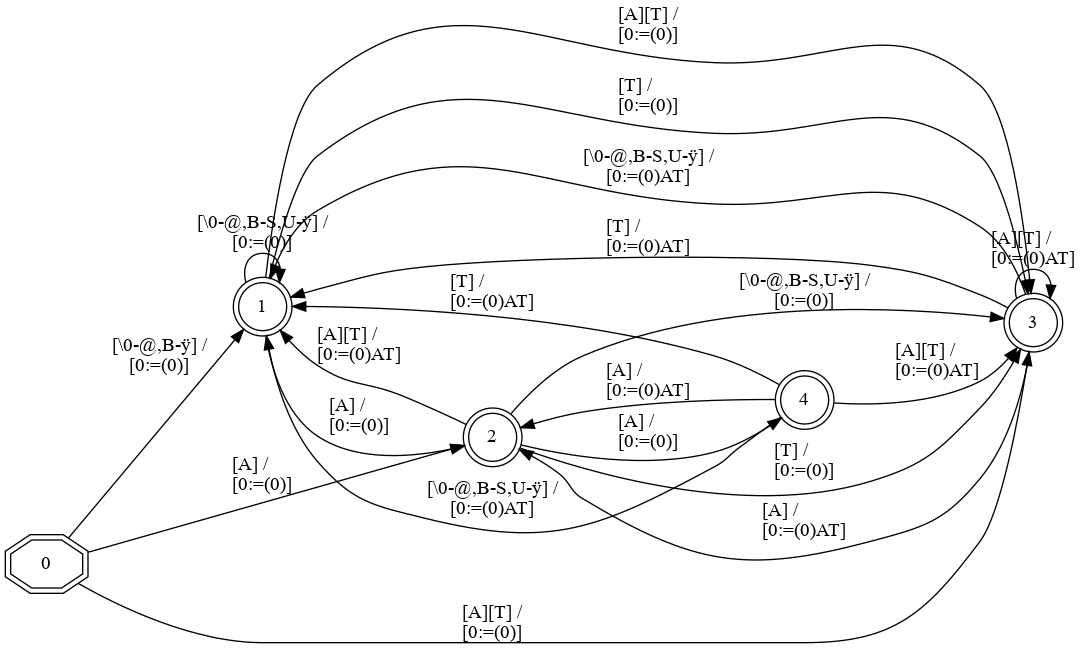
\includegraphics[width=0.9\textwidth]{images/sst.png}
  \caption{SST of the simple approximate Kleenex program}
  \label{fig:sst}
\end{figure}

\begin{figure}[!hb]
  \centering
  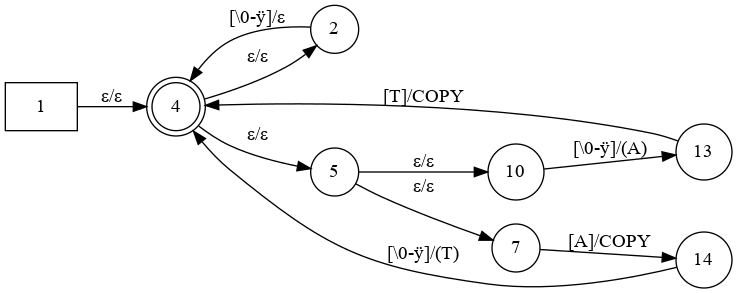
\includegraphics[width=0.9\textwidth]{images/opt.png}
  \caption{An optimized version of the OFT}
  \label{fig:opt}
\end{figure}

\subsection{Ideas for improving Kleenex}
% TODO: write properly

The result of the $k$-fold rewrite of a core Kleenex program, as described in
Troelsen's thesis~\cite{troelsen2016approximate} and exemplified in
Section~\ref{sec:approx-kleenex}, is proved in his thesis to be possible to
execute in time $\mathcal{O}(mnk)$ by determinization to an SST, where $n$ is
the size of the input string and $m$ is the size of the transition relation of
the corresponding NFST. This is proved by arguing that the growth of the number
of transitions in the transducer is in the order $\mathcal{O}(mk)$ (for $k>0$),
since the transformation adds $k$ new transitions to the transducer for each
existing transition and at most a constant number of additional transitions for
each of these new transitions, depending on the error metric. The
aforementioned time bound then follows from the result
in~\cite{grathwohl2016kleenex} that the SST can be implemented to execute in
time $\mathcal{O}(mn)$.

%This utilizes the results of Theorem 1 and Corollary 1 in the POPL paper.

Grathwohl et al.~\cite{grathwohl2016kleenex} also prove that for an oracle
machine of size $m$, i.e. an NFST with $m$ transitions, there is a semantically
equivalent SST with $\mathcal{O}(2^{m \log m})$ states. A corollary to this is
that for a core Kleenex program with a corresponding transducer of size $m$,
allowing approximate matches with up to $k$ errors, there is an SST with
$\mathcal{O}(2^{mk \log mk})$ states. Thus, the number of states in the SST
resulting from the rewriting of core Kleenex and following determinization of
the NFST, is exponential in $k$.

This seems to suggest a potential cause of the increased compilation times when
using approximate matching in Kleenex and the very large output programs that
it generates. Thus, one may be interested in exploring ways to avoid the
increase in size of the NFST.

% TODO: Talk about the inconvenient way that counting errors is represented by
% directly encoding it in the grammar rather than simply counting the errors.

% Theorem 2 from the POPL paper states that for an oracle machine of size $m$,
% i.e. the size of the transition relation, there is a (semantically equivalent)
% SST with $O(2^{m \log m})$ states.

% Counters, implemented as optimization in the implementation vs. updating the
% automata models.

\subsubsection{Tagged automata}

In his bachelor's thesis~\cite{enevoldsen2015pattern}, Sune Enevoldsen uses the
concept of a tagged automaton, based on work by Ville
Laurikari~\cite{laurikari2000nfas, laurikari2001efficient} and inspired by
Levenshtein automata~\cite{schulz2002fast}, to do approximate regular string
matching. This model was originally introduced to solve the problem of
extracting the position of matches for subexpressions of a regular expression,
however Laurikari also suggests its application to approximate matching.

A nondeterministic automaton with tagged transitions, or a tagged NFA, is a
finite automaton extended with a set of tags which may be set or modified on
each transition in the transition relation. The idea is to use these tags as
counters which keep track of the allowed number of errors, e.g. insertions,
deletion, and substitutions. A formal definition follows:

% Thus, the tagged automata for a given regular expression $RE$ will accept the
% strings in $\mathcal{L}(RE)$ as well as any string that is within a certain
% error distance of a string in $\mathcal{L}(RE)$.

\begin{definition}[NTA]
  A \emph{nondeterministic tagged automaton} (NTA) is a structure
  $(\Sigma, Q, q^s, F, T, t_0, \Delta)$, where $\Sigma$ is a finite alphabet,
  $Q$ is a finite set of states, $q^s$ is the initial state, and
  $F \subseteq Q$ is the set of final states. $T$ is a set of possible tag
  values, $t_0$ is the initial tag value and $\Delta$ is the transition
  relation
  \[
    \Delta \subseteq Q \times T \times \Sigma[\epsilon] \times Q \times T \;.
  \]
\end{definition}

The transition relation can also be described in terms of functions on tag
values. For each transition from state $p$ to state $q$ on input symbol $a$,
define a function $U_{p,a,q}$ from the set of tags $T$ to sets of tags. For the
purpose of approximate matching, and as in Enevoldsen's thesis, these functions
will always return just a singleton set or the empty set. Such a tag function
may ignore the tag, i.e. just return a singleton set of the given unchanged
tag, it may set a new tag independent of the current tag value, or it may set a
tag value depending on the current value. In particular, if
$U_{p,a,q}(t) = \emptyset$, then the automaton cannot transition from state $p$
to state $q$ on symbol $a$ when the tag $t$ is set.

We mark the transitions in the automaton with the tag functions, or just with
the new tag value if the function does not depend on its argument.

To use this automaton for approximate regular string matching using the
Levenshtein distance metric, we can set $T = \mathbb{N}^3$ and $t_0 =
[0,0,0]$. Thus, when entering a subexpression which allows a specified number
of substitutions, insertions, and deletions, the ingoing transition can set the
tag to the allowed errors. Similarly when leaving the subexpression, the tag
can be reset to $[0,0,0]$. For a mismatch, the tag function will be
\[
  M([m,i,d]) =
  \begin{cases}
    \emptyset     & \text{if } m = 0 \\
    \{[m-1,i,d]\} & \text{otherwise}
  \end{cases}
\]
and analogously for insertions, denoted $I$, and deletions, denoted $D$.

Thus, for Thompson's construction~\cite{thompson1968programming}, the case for
a literal character regular expression $a \in \Sigma$ is changed to the
following, where $\bar{a}$ denotes a symbol $c \in \Sigma \setminus \{a\}$ and
$.$ denotes any symbol in the alphabet:

\begin{center}
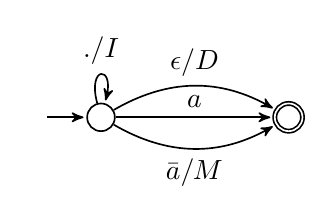
\begin{tikzpicture}[->,>=stealth',shorten >=1pt,auto,node distance=2.0cm,
  semithick, main/.style={circle,draw,minimum width=10pt}]
    \node (q0) {};
    \node[main] (q1) [right = 5mm of q0] {};
    \node[main,accepting] (q2) [right = of q1] {};
    \path (q0) edge (q1)
    (q1) edge [loop above] node {$./I$}
    (q1) edge node {$a$} (q2)
    (q1) edge[bend left] node {$\epsilon/D$} (q2)
    (q1) edge[bend right] node[below] {$\bar{a}/M$} (q2);
\end{tikzpicture}
\end{center}

For the sake of simplicity, consider now just the mismatch error type. Extend
the notion of tagged automata to transducers in the straightforward way,
e.g. by added the output alphabet to the tagged automaton and modifying the
transition relation to include output, as follows:
\[
  \Delta \subseteq Q \times T \times \Sigma[\epsilon] \times \Gamma[\epsilon]
  \times Q \times T
\]

One could transform an NFST for exact matching to a tagged NFST by translating
the core Kleenex term $N ::= \mathtt{a}N'$ to the following transitions in the
NFST:

\begin{center}
  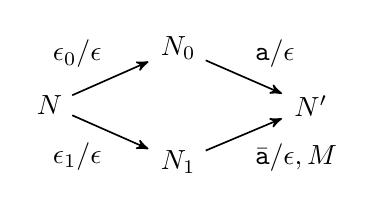
\begin{tikzpicture}[->,>=stealth',shorten >=1pt,auto,semithick,
    main/.style={minimum width=10pt}]
    \node (q0) {$N$};
    \node (q0a) [above right = 2mm and 10mm of q0] {$N_0$};
    \node (q0b) [below right = 2mm and 10mm of q0] {$N_1$};
    \node (q1) [below right = 2mm and 10mm of q0a] {$N'$};
    \path (q0) edge node {$\epsilon_0/\epsilon$} (q0a)
    (q0) edge node [below left] {$\epsilon_1/\epsilon$} (q0b)
    (q0a) edge node {$\mathtt{a} / \epsilon$} (q1)
    (q0b) edge node [below right] {$\bar{\mathtt{a}}/\epsilon, M$} (q1);
  \end{tikzpicture}
\end{center}

Here the $M$ in $\bar{\mathtt{a}}/\epsilon, M$ denotes the tag function on the
transition, which decrements the number of allowed mismatches by one.

Continuing the example from Section~\ref{sec:approx-kleenex}, a tagged
transducer for the described core Kleenex program, accepting the language $a^*$
with a given number of allowed substitutions, may be realized as shown in
Figure~\ref{fig:tagged-transducer}.

\begin{figure}[!hb]
  \centering
  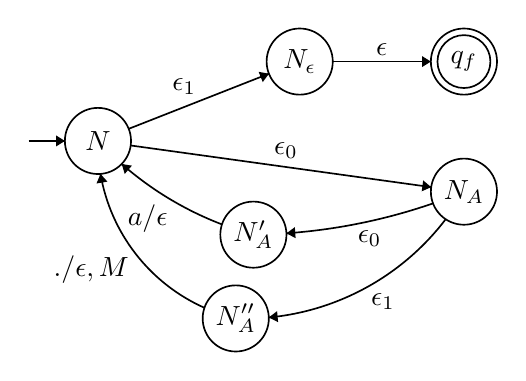
\begin{tikzpicture}[>=stealth',semithick,scale=0.14]
  \tikzstyle{every node}+=[inner sep=0pt,minimum width=10pt]
  \draw [black] (26.3,-22.6) circle (3);
  \draw (26.3,-22.6) node {$N$};
  \draw [black] (44.6,-15.4) circle (3);
  \draw (44.6,-15.4) node {$N_\epsilon$};
  \draw [black] (59.5,-15.4) circle (3);
  \draw (59.5,-15.4) node {$q_f$};
  \draw [black] (59.5,-15.4) circle (2.4);
  \draw [black] (59.5,-27.2) circle (3);
  \draw (59.5,-27.2) node {$N_A$};
  \draw [black] (38.8,-38.7) circle (3);
  \draw (38.8,-38.7) node {$N''_A$};
  \draw [black] (40.4,-31.1) circle (3);
  \draw (40.4,-31.1) node {$N'_A$};
  \draw [black] (47.6,-15.4) -- (56.5,-15.4);
  \fill [black] (56.5,-15.4) -- (55.7,-14.9) -- (55.7,-15.9);
  \draw (52.05,-14.9) node [above] {$\epsilon$};
  \draw [black] (29.09,-21.5) -- (41.81,-16.5);
  \fill [black] (41.81,-16.5) -- (40.88,-16.33) -- (41.25,-17.26);
  \draw (34.12,-18.47) node [above] {$\epsilon_1$};
  \draw [black] (29.27,-23.01) -- (56.53,-26.79);
  \fill [black] (56.53,-26.79) -- (55.8,-26.18) -- (55.67,-27.17);
  \draw (43.36,-24.27) node [above] {$\epsilon_0$};
  \draw [black] (57.844,-29.699) arc (-37.28549:-84.6053:22.872);
  \fill [black] (41.8,-38.61) -- (42.64,-39.04) -- (42.55,-38.04);
  \draw (52.15,-36.34) node [below] {$\epsilon_1$};
  \draw [black] (56.695,-28.262) arc (-70.92823:-85.99078:51.775);
  \fill [black] (43.4,-30.98) -- (44.23,-31.42) -- (44.16,-30.42);
  \draw (50.94,-30.68) node [below] {$\epsilon_0$};
  \draw [black] (35.963,-37.737) arc (-114.02842:-170.32022:16.304);
  \fill [black] (26.53,-25.59) -- (26.17,-26.46) -- (27.16,-26.29);
  \draw (29.16,-34.26) node [left] {$./\epsilon,M$};
  \draw [black] (37.549,-30.17) arc (-110.92075:-131.24549:30.097);
  \fill [black] (28.45,-24.69) -- (28.73,-25.59) -- (29.38,-24.84);
  \draw (30.81,-28.33) node [below] {$a/\epsilon$};
  \draw [black] (20,-22.6) -- (23.3,-22.6);
  \fill [black] (23.3,-22.6) -- (22.5,-22.1) -- (22.5,-23.1);
  \end{tikzpicture}
  \caption{Conceptual visualization of a tagged transducer for core Kleenex
    programmed described and rewritten in Section~\ref{sec:approx-kleenex}.}
  \label{fig:tagged-transducer}
\end{figure}

Compare this to the transducer for the rewritten core Kleenex program, shown in
Appendix~\ref{app:approx-kleenex-example}. Furthermore, this tagged transducer
is of a fixed size independent of $k$, compared to the linear growth of the
rewritten program.

It may be possible to simulate a tagged transducer like a regular transducer,
using path-tree simulation, by extending the state of each leaf of the path
tree to include the number of allowed mismatches in that state. A leaf in the
path tree will then be able to step on a given input symbol according to the
transition relation, if the tag function maps the current tag to a nonempty
set, the single element of which will then be the new tag, otherwise the path
will fail.

The question still remains, whether it is possible to determinize such an
automaton to an SST and how many states it would generate. Following the
argument in \cite{soholm2015ordered}, there is a finite number of reduced path
trees, ignoring outputs, and since the value of $k$ for any given leaf is also
bounded, there is also a finite number of reduced path trees with associated
error counts. Thus, it should be possible to determinize these into a streaming
string transducer, that is, a deterministic automaton with abstract states
corresponding to the reduced path trees as states, transitions representing the
changes to the path tree during simulation, and registers storing the outputs
associated with each node in the path tree. The size of such an SST will have
to be investigated in future work.


\subsubsection{Scanning for subpatterns}

Another potential idea for improving the performance of approximate Kleenex is
to select subpatterns to search for, as also used in NR-grep and discussed
in~\cite{navarro2001nr}. Specifically for approximate Kleenex, where the size
of the SST appears to be a critical issue, compiling only a shorter and perhaps
simpler subpattern to an SST could significantly reduce the determinization
overhead. A good choice for a subpattern may be significantly simpler, yet its
occurrence in the text could yield a high probability for an actual match of
the whole pattern, depending on the assumptions made about the text. This
potential match can then be verified, e.g. by simulating the transducer using
path-tree simulation.

For example, consider the Kleenex program for the ranges benchmark case:
\texttt{(/[ACGT]/\{5,15\} /TGCAAGCGTTAAT/)<$k$>}, which could only be compiled
for $k\leq1$. Compiling only the pattern \texttt{/TGCAAGCGTTAAT/}, with errors
allowed, will significantly reduce the size of the SST, but is expected to
still provide a good indication for the probability of a match

As mentioned NR-grep, among others, uses this techniques and
\cite{navarro2001nr} describes techniques for selecting an optimal subpattern
under some simplifying assumptions about the text characters.

%%% Local Variables:
%%% mode: latex
%%% TeX-master: "main"
%%% End:

\section{Conclusion}
As long as the patterns are simple enough so that Kleenex compiles a not too
large executable, it seems to be able to compete with or outperform the other
tools we have tested, with NR-grep being the biggest difference, but it does
have an unfair advantage in using the input with newlines.


\clearpage
\bibliographystyle{plain}
\bibliography{tipl}

\clearpage
\appendix
\section{Example of transducer for approximate Kleenex program}
\label{app:approx-kleenex-example}

\begin{figure}[!ht]
  \begin{subfigure}[t]{1\textwidth}
    \centering
    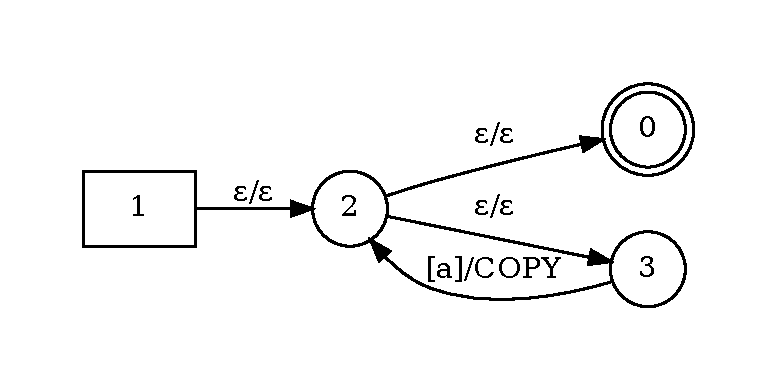
\includegraphics[width=0.5\textwidth]{images/as_exact.pdf}
    \caption{Transducer for the original program.}
  \end{subfigure}
  ~
  \noindent\makebox[\textwidth]{%
  \begin{subfigure}[t]{1.4\textwidth}
    \centering
    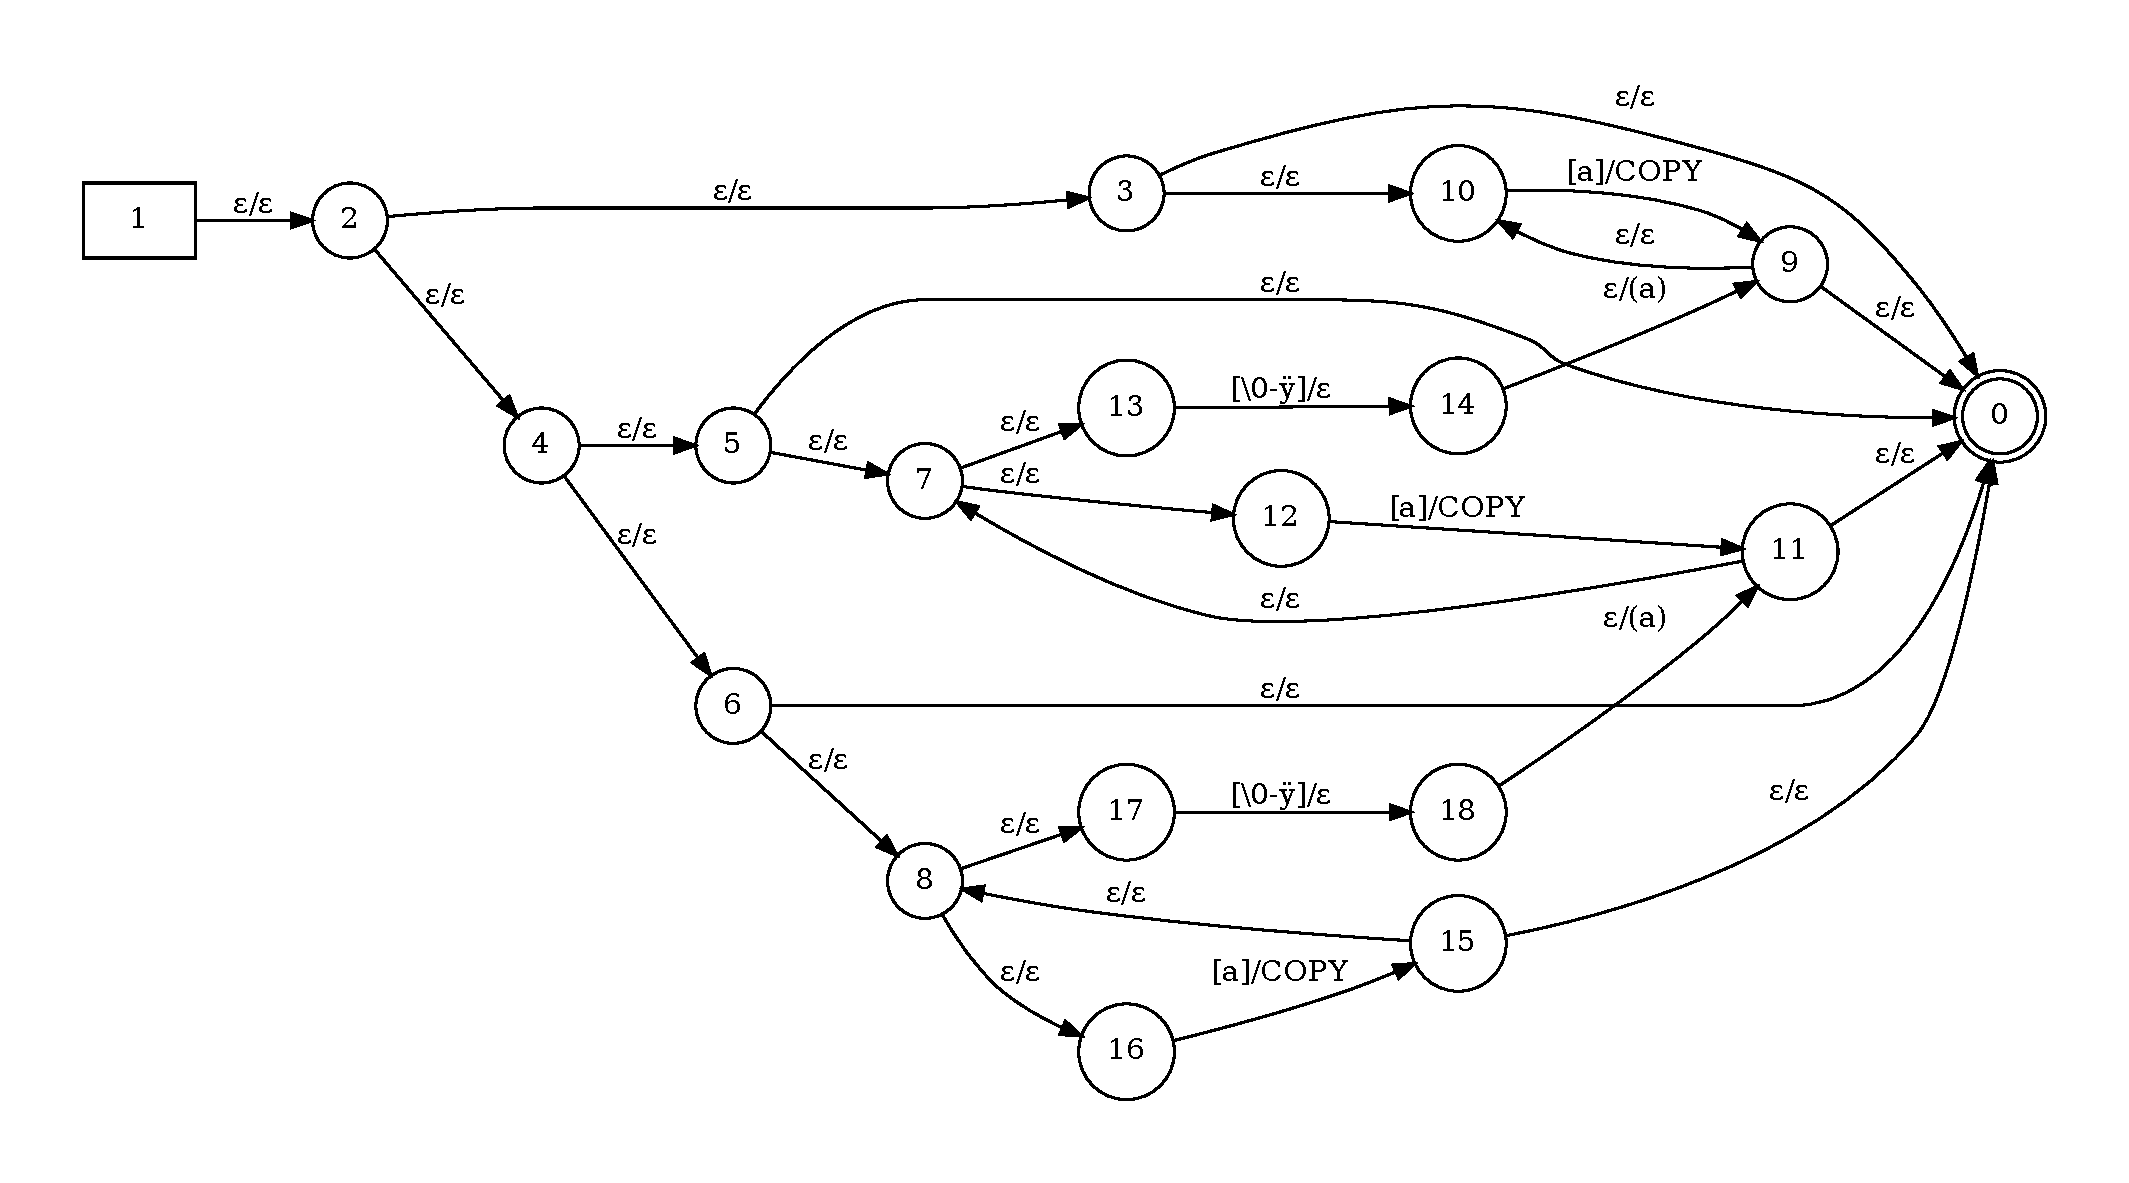
\includegraphics[width=\textwidth]{images/as_k2_hamming.pdf}
    \caption{Transducer for the rewritten program.}
  \end{subfigure}}
  \caption{Visualization of transducers for the original Kleenex program
    accepting exactly $a^*$ and the rewritten program accepting $a^*$ with
    $k=2$ errors using Hamming distance.}
\end{figure}

%%% Local Variables:
%%% mode: latex
%%% TeX-master: "main"
%%% End:


\end{document}

%%% Local Variables:
%%% mode: latex
%%% TeX-master: t
%%% End:
